%
% File acl2015.tex
%
% Contact: car@ir.hit.edu.cn, gdzhou@suda.edu.cn
%%
%% Based on the style files for ACL-2014, which were, in turn,
%% Based on the style files for ACL-2013, which were, in turn,
%% Based on the style files for ACL-2012, which were, in turn,
%% based on the style files for ACL-2011, which were, in turn, 
%% based on the style files for ACL-2010, which were, in turn, 
%% based on the style files for ACL-IJCNLP-2009, which were, in turn,
%% based on the style files for EACL-2009 and IJCNLP-2008...

%% Based on the style files for EACL 2006 by 
%%e.agirre@ehu.es or Sergi.Balari@uab.es
%% and that of ACL 08 by Joakim Nivre and Noah Smith

\documentclass[11pt]{article}
\usepackage{acl2015}
\usepackage{times}
\usepackage{booktabs}
\usepackage{latexsym}
\usepackage{graphicx}
\usepackage{array,etoolbox}
\usepackage{tikz}
\preto\tabular{\setcounter{magicrownumbers}{0}}
%\newcommand{\circlednumber}[1]{\raisebox{.5pt}{\textcircled{\raisebox{-.9pt} {#1}}}}
\newcommand*\circlednumber[1]{\tikz[baseline=(char.base)]{
    \node[shape=circle,draw,inner sep=1pt, minimum size=1pt] (char) {#1};}}
\newcounter{magicrownumbers}
\def\rownumber{}
%\setlength\titlebox{5cm}

% You can expand the titlebox if you need extra space
% to show all the authors. Please do not make the titlebox
% smaller than 5cm (the original size); we will check this
% in the camera-ready version and ask you to change it back.


\title{Fusion Techniques for Named Entity Recognition and Word Sense Induction and Disambiguation}

\author{First Author\\
  Affiliation / Address line 1 \\
  Affiliation / Address line 2 \\
  Affiliation / Address line 3 \\
  {\tt email@domain} \\\And
  Second Author \\
  Affiliation / Address line 1 \\
  Affiliation / Address line 2 \\
  Affiliation / Address line 3 \\
  {\tt email@domain} \\}

\date{}

\begin{document}
\maketitle
\begin{abstract}
In this paper we explore the use of well-known multi-modal fusion techniques to solve two prominent Natural Language Processing tasks. Specifically, we focus on solving Named Entity Recognition and Word Sense Induction and Disambiguation by applying feature-combination methods that have already shown their efficiency in the multi-media analysis domain. We present a series of experiments employing fusion techniques in order to combine textual linguistic features. Our intuition is that by combining different types of features we may find semantic similarities among words at different levels. Thus, the combination (and recombination) of these levels may yield gains in terms of performance.
% To our knowledge, employing these techniques has not been studied for the tasks we address in this paper. 
We test the proposed fusion techniques on three datasets for named entity recognition and two for word sense disambiguation and induction. Our results show that the combination of textual features indeed improves the performance compared to single feature and the trivial feature concatenation.
\end{abstract}


\section{Introduction}

Named Entity Recognition (NER) and Word Sense Induction and Disambiguation (WSI/WSD) requires, as other learning tasks, textual features to represent the similarities between words to discern between different words' meanings. 

NER goal is to automatically discover, within a text, mentions that belong to a well-defined semantic category. The classic task of NER involves entities of type Location, Organization, Person and Miscellaneous. The task is of great importance for more complex NLP systems, e.g, relation extraction, opinion mining. The two historical solutions to NER are one of the following: via matching patterns created manually or extracted semi-automatically; or by training a supervised machine learning algorithm with large quantities of annotated text. The latter being the currently more popular solution to this task.




%In the classic case of NER, we need to determine, given its context, whether a word is referring a person, a location, an organization or another miscelaneous entity. On the other hand, in WSI/WSD the goal is to determine and assign the specific meaning of a target word, again based on its context.

Word Sense Induction and Disambiguation entails two closely related tasks\footnote{Even though these tasks are closely related, they are independent from one another. Still, in this paper we consider them to be a single one.}. WSI aims to automatically discovering the set of possible senses for a target word given a text corpus containing several occurrences of said target word. Meanwhile, WSD takes a set of possible senses and determines the most appropriate sense for each instance of the target word according to the instance's context. WSI is usually approached as an unsupervised learning task, i.e., a cluster method is applied to the words occurring in the instances of a target word. Then, the groups found are interpreted as the senses of the target word. The WSD task is usually solved with knowledge-based approaches, based on BabelNet [] or WordNet [] or more recently with supervised models which require large quantities of annotated data.

As stated before, both tasks rely on features extracted from the text. Usually, these representations are obtained from the sourrounding context of the words of the an input corpus. Mainly,  two types of representations are typically used according to their nature. We call these features lexical and syntactical. 	The first type requires no extra information that that contained already in the analyzed text itself. It consists merely on the tokens sourrounding a word, i.e., those tokens that come before and after in a fixed window of a studied token. The second type, syntactical features, is similar to lexical representation in that we also consider as features the tokens that appear next to the corpus' words. Nonetheless, it requires a a larger degree of language understanding. In particular, these features are based on part of speech tags, phrase constituents information, as well as syntactical interaction between words or syntactical dependencies.

Other features, specific to one task or another may also be employed. For example, in NER, some standard features used in the literature include whether a word begins with an upper-case letter, the type of prefix and suffix of the word itself as well as the context words, and so on.

%In the latter case, as with any supervised model, we need to first define a set of features that will better represent each token. In this work, we make use of three different types of linguistic data, that is, (1) lexical co-occurrence, (2) grammatical dependency relations and (3) constituent-tree branch membership to try and solve the NER task. More importantly, we propose a fusion framework that uses different methods to combine these three sources of information (among others) into a single representation model.

Most of the approaches in the literatire dealing with these task use each of these features independently or stacked together as concatenated columns in an input representation space matrix. In the latter case, features are used without regards to their nature. 

The intuition of the present work is that word similarities may be found at different levels according to the type of features employed. In order to exploit these similarities, we look into multimedia fusion methods. These techniques consider the integration of multimodal representations, or their corresponding similarities, or  decisions product of models trained with these features in order to perform an analysis task.  Particularly, we try to mutually complement independent representations by utilizing said fusion techniques to combine (or fuse) features in the hope of improving the performance of the tasks of interest, specially compared to the use of features independently. 

Fusion techniques have previously shown their efficiency, mainly on image-related tasks, where there is a need to model to leverage the relation  between images and text extracts.
%
%For example, in information retrieval (Ah-Pine et al., 2015), lexicon learning (Vulic et al., 2016), coreference resolution (Eisenstein and Davis, 2007); different types of representations (different modalities) can be combined in order to take advantage of the complementarity existing among them. 
%
In contrast, in this work we consider the textual features as coming from different modalities. The main contribution of this work is to assess the effectiveness of simple yet untested techniques to combine classical and easy to obtain textual features. 

The rest of the paper is organized as follows: in section 2, we go into further detail about fusion techniques as well as its application in the NLP domain. We introduce the operator that we use in the followed methodology of our experiments, described in section 3. Then, in section 4 we show the effectiveness of the presented methods by testing them on NER and WSI/WSD and their respective datasets. Finally, in section 5 we present our conclusions and future directions to explore. A more general overview on fusion for multimedia analysis can be found in \cite{AtreyHEK10}.

\section{Background and Related Work}
 
We first describe below the fusion techniques we use in our methodology as well as relevant use cases where they have been employed. Then, we focus exclusively on fusion techniques applied to NLP tasks, which is the general domain of the two tasks (NER and WSI/WSD) we focus on this paper.                                                                                                                 
\subsection{Multimodal Fusion Techniques}
Multimodal fusion is a popular technique used in multimedia anlysis tasks. Formally, these techniques integrate multiple media features, the affinities among these attributes or the decisions obtained from systems trained with said features, to obtain rich insights about the data being used and thus to solve a given analysis  task \cite{AtreyHEK10}. We note that these techniques come at the price of augmenting the complexity of a given system by increasing or reducing the sparsity of a given feature matrix.


In recent multi-modal fusion literature we can discern two main types of techniques: early fusion and late fusion. 
\paragraph{Early Fusion}
Early fusion is the most widely used method. The principle is simple: we take both modal features and concatenate them into a single representation matrix. More formally, we consider two matrices  that represent different modality features each  over the same set of individuals. To perform early fusion we concatenate them column-wise, such that we form a new matrix having the same number of lines but increasing the number of columns to the sum of the number of columns of both matrices. The matrices may also be weighted as to control the influence of each modality.

The main advantage of early fusion is that a single unique model is fitted while leveraging the correlations among the concatenated features. The method is also easy to integrate into an analysis system. The main drawback is that we increase the representation space and may make it harder to fit models over it.
%

%   of shape $(n, m + p)$. Following the literature notation of [vulic], the early fusion representation matrix EF is defined as:
%\begin{equation}
%EF = \alpha \times X_1 || (1 - \alpha) \times X_2
%\end{equation}

%where $||$ represents the column-wise concatenation operation and α is the parameter that determines the contribution of each modality. 
%
Early fusion has been employed in several multi-modal tasks. For example, [?]. 
\paragraph{Late Fusion}
In contrast to early fusion, in late fusion the combination of multimodal features are generally performed at the decision level, i.e., using the output of independent models trained  each with an unique set of features \cite{ClinchantAC11}. In this setting,  decisions produced by each model are combined into a single final result set.
%
The methods used to combine preliminary decisions usually involve one of two types: rule-based (where modalities are combined according to domain-specific knowledge) or linear fusion (e.g., weighting and then adding or multiplying both matrices together). This type of fusion is very close to the so-called ensemble methods in the machine learning literature, namely the stacking methods.
%
Late fusion combines both modalities in the same semantic space. In that sense,  we may also combine modalities via an affinity representation instead of final decision sets. In other words, we can combine two modality matrices by means of their respective similarities. A final representation is then usually obtained by adding the weighted similarity matrices.
%

The advantages of late fusion include the combination of features at the same level of representation (either the fusion of decisions or similarity matrices). Also, given that independent models are trained separately, we can chose which algorithm is more adequate for each type of
features.
\paragraph{Cross-media Similarity Fusion}

%
In \cite{Ah-PineCC15}, cross-media similarity fusion is defined and employed to propagate a single modality
similarity into a second modality similarity matrix. Specifically, the procedure tries to bridge the semantic
gap between textual and visual information by using the most similar objects in the textual similarity matrix as a proxy to transfer the information to the visual similarity matrix. In this paper we also experiment with this type of fusion.

\paragraph{Hybrid Fusion}
We may leverage the advantages of the previous two types of fusion techniques by combining them once more in a hybrid setting. As described in \cite{AtreyHEK10,yu2014informedia}, the main idea is to simultaneously combine features at the feature level, i.e., early fusion, and at the same semantic space or decision level. Nonetheless, they define a specific type of hybrid fusion. In this paper, we adopt a looser definition of hybrid fusion. That is, we perform hybrid fusion by leveraging the combination of the fusion strategies described before.
%In a general sense,
%having two similarity matrices $S_1$ and $S_2$ defined as above, we define the cross-media similarity fusion as:
%
%\begin{equation}
%XF = \mathbf{K}(S_1, k) \cdot S_2
%\end{equation}
%
%where $\mathbf{K}$ is a row-wise function that keeps only the top-k values of the similarity matrix S 1 and
%assigns zero to the rest of the line.

%In Table [] we show a synthetic table with the literature works on fusion cited in this section. We present the task solved by each contribution, the type of fusion used, the modalities involved and finally the performance gain obtained while using the fusion techniques.

%\subsection{NER and WSI/WSD}
%Previously we introduced NLP works that made use of a fusion strategy to improve a single modality system. Nonetheless, and to the best of our knowledge, there is no work that addresses NER directly while using fusion techniques from the multimedia analysis domain.


In the following section we present the core of the work presented in this paper. We consider the first three types of fusion techniques (early fusion, late fusion and cross-media fusion) as the building blocks to the experiments we conduct.  While we work with a single modality, i.e., textual data, we consider the different kinds of features extracted from it as distinct modalities. Our intuition being that the semantic similarities among words in these different spaces can be combined in order to exploit the latent complementarity between the lexical and syntactical representations. The fusion should therefore improve the performance of the NLP tasks at hand, NER and WSI/WSD.

Our first goal is to assess the effectiveness of the classic fusion methods and then, as a second goal, to propose new combinations that yield better outcomes in terms of performance than the simpler approaches. The new combinations are found empirically. Nonetheless, as we will show, their effectiveness replicates within different datasets and NLP tasks. This kind of fusion combinations is somewhat similar to previously employed approaches which join early fusion with cross-media fusion operators to construct random-walk based fusion methods \cite{Ah-PineCC15,GialampoukidisM16}. These techniques iterate over the fusion operators several times in the hopes of better propagating useful information across modalities. Still, we do not perform any kind of iteration. Our approaches perform a single step to obtain a representation matrix.

In the following section we formally describe the fusion techniques described before, which we employ in the next section. Also, we also delineate the procedure followed in our experiments. 

\begin{figure*}
\centering
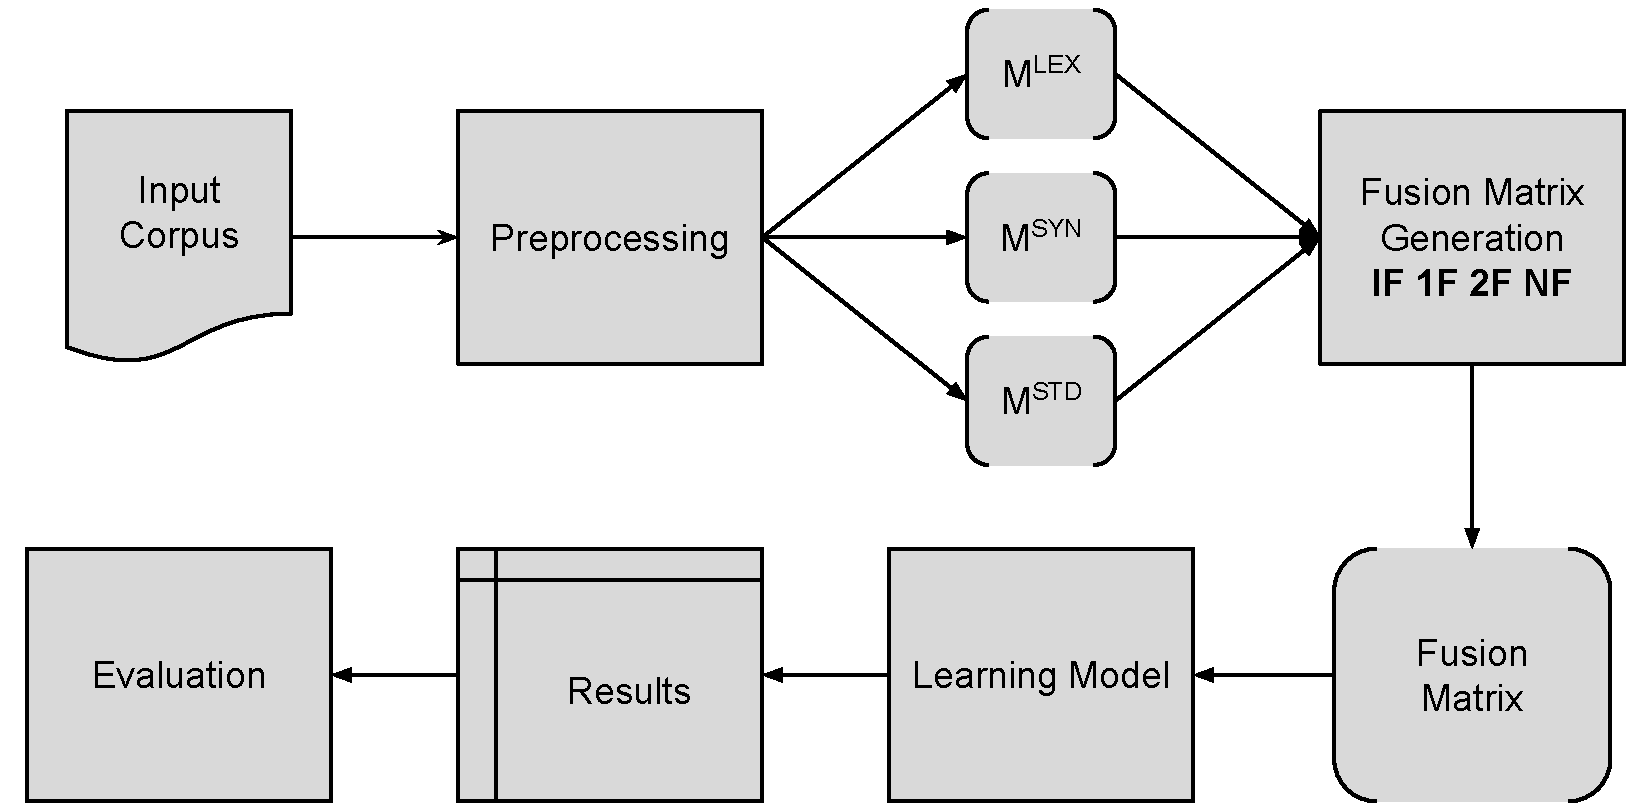
\includegraphics[width=0.85\linewidth]{img/diag_metodo}
\caption{}
\label{fig:diagmetodo}
\end{figure*}

The experiments we carry on consist in generating matrices that will serve as input to a learning algorithm in order to solve NER and WSI/WSD. These input feature matrices are be based upon lexical, syntactical, or other types of representation. 

\subsection{Fusion Strategies}
We begin by presenting a  formal definition of the fusion techniques employed and described in the previous sections. We define early fusion, late fusion and cross-media fusion as follows:
\paragraph{Early Fusion}
\begin{equation}
E_\alpha(A,B) = \mathbf{hstack}(\alpha\cdot A , (1-\alpha)\cdot B)
\end{equation}
\paragraph{Late Fusion}
\begin{equation}
L_\beta(A,B) = \beta \cdot A + (1 - \beta)\cdot B
\end{equation}
\paragraph{Cross-media Fusion}
\begin{equation}
X_{\gamma}(A,B) = \mathbf{K}(A,\gamma) \times B
\end{equation}

%\vspace{.3cm}

Parameters $A$ and $B$ are input matrices. They may initially represent, for example,  the lexical ($M^{LEX}$) or syntactical based ($M^{SYN}$) features matrix, or their  corresponding similarity matrices, $S^{LEX}$ and  $S^{SYN}$, ~respectively. In a broader sense, matrices $A$ and $B$ may represent any pair of valid\footnote{Valid in terms of having compatible shapes while computing a matrix sum or multiplication.} fusion matrices. 

In early fusion, $E_\alpha(A,B)$, the matrices $A$ and $B$ are combined together via a concatenation function $\mathbf{hstack}$ which joins both of them column-wise. The $\alpha$ parameter controls the importance of each matrix.

Regarding late fusion $L_\beta(A,B)$, the  $\beta$ parameter determines again the importance of the  matrix $A$,  and consequently also the relevance of matrix $B$.

In cross late fusion $X_\gamma(A,B)$, the $\mathbf{K}(\cdot)$ function keeps the top-$\gamma$ closest words (columns) to each word (lines) while the rest of the values are set to zero.

Using the previously defined operators, we carry out four levels of experiments: 
\begin{enumerate}
\item \textbf{Independent Features}: in this phase we consider the modalities independently as input to the learning methods. For instance, we may train a model for NER using only the lexical features matrix $M^{LEX}$.
\item \textbf{First-degree Fusion}: we  consider the most three elementary fusion techniques by themselves (early fusion, late fusion, cross-media fusion) without any recombination.  These experiments, as well as those from the previous level, serve as the baselines we set to surpass in order to show the efficacy of the rest of the fusion approaches.
As an example, we may obtain a representation matrix by performing an early fusion between the lexical matrix and the syntactical features matrix: $E(M^{LEX}, M^{SYN})$.
\item \textbf{Second-degree Fusion}: here we recombine the outputs of the previous two levels with the elementary techniques. This procedure then yields a recombination of "second-degree" among fusion methods. A second-degree fusion would be an early fusion of the lexical feature matrix with a cross-media fusion, expressed as $E(M^{LEX}, X(S^{STD}, M^{STD}))$.   
\item \textbf{N-degree Fusion}: in this last level we follow a similar approach to the previous level by coombining the output of the second-degree fusion level multiple times with other second-degree fusion outputs. As an example, the equation $E(L(M^{STD}, X(S^{STD}, M^{STD})), \allowbreak L(M^{LEX}, X(S^{SYN}, M^{LEX})))$  denotes the early fusion between two operations: (1) a late fusion between a lexical-features matrix and a cross-media fusion, and (2),  another late fusion consisting of a standard-features matrix (this matrix is detailed below)  and a cross-media fusion. In general, we determine a n-degree fusion empirically. That is to say, we look at the performance of second-degree fusions and try to improve the performance of the systems by recombining the fusion outputs via a n-degree combination. This process is in fact applied during the second-degree fusions also. 
\end{enumerate}   
\subsection{Feature Matrices}
In the previous subsection we presented the fusion operators used in our experiments. Below we detail the three types of features used to describe the words of the corpus tested.
\paragraph{Lexical Matrix (LEX)}
For each token in the corpus, we use a lexical window of two words to the left and two words to the right, plus the token itself. Specifically, for a target word $w$, its lexical context is $(w_{-2}, w_{-2}, w, w_{+1}, w_{+2})$. This type of context features is typical for any system studying the sourroundings of a word, i.e., using a distributional approach.
% We retake the example phrase from \cite{LevyG14}, the lexical-based features of the phrase \textit{Australian scientist discovers start with telescope}, are shown in Table \ref{tab:lex-contexts}.
%\begin{table*}[ht]
%\centering
%\begin{tabular}{ll}
%\hline 
% \textbf{Word} & \textbf{Features} \\ 
%\hline 
%Australian & word:Australian, word+1:scientist, word+2:discovers\\ 
%scientist  &  word-1:Australian, word:scientist, word+1:discovers, word+2:star\\ 
%discovers & word-2:Australian, word-1:scientist, $\dots$, word+2:telescope \\ 
%star & word-2:scientist, word-1:discovers, word:star, $\dots$, word+2:telescope \\ 
%with & word-2:discovers, word-1:star, word:with, word+1:telescope \\ 
%telescope  &  word-2:star, word-1:with, word:telescope \\ 
%\hline \
%\end{tabular} 
%\label{tab:lex-contexts}
%\caption{Lexical features corresponding to the phrase \textit{Australian scientist discovers start with telescope}.}
%\end{table*} 

\paragraph{Syntactical Matrix (SYN)}
Based on the syntactic features used in   \cite{LevyG14,Panchenko2017}, we derive contexts based on the syntactic relations a word participates in, as well as including the part of speech (PoS) of the arguments of these relations. Formally, for a word $w$ with modifiers $m_1, \dots, m_k$ and their corresponding PoS tags $p^m_1, \dots, p^m_k$; a head $h$ and its corresponding PoS tag $p^h$, we consider the context features $(m_1, p_{m_1}, lbl_1), \dots, (m_k, p_{m_k}, lbl_k), \allowbreak (h,p_h,lbl\_inv_h)$. In this case, $lbl$ and $lbl_inv$ indicate the label of the dependency relation and its inverse, correspondingly. Using syntactic dependencies as features should yield more specific similarities, closer to synonymy, instead of the broader topical similarity found through lexical contexts.
%For the phrase \textit{Australian scientist discovers start with telescope} the dependency-based context is shown in Table \ref{tab:syn-contexts}.
\paragraph{NER Standard Features Matrix (STD)}

The features used for NER are based roughly the same as those used for the same task in \cite{Daume2006,Balasuriya2009}. The feature set consists of: the word itself, whether the word begins with capital letter, prefix and suffix up to three characters (within a window of two words to the left and two words to the right), and the PoS tag of the current word. These features are considered to be standard in the literature. We note that the matrix generated with these features is exclusively used in the experiments regarding NER.	

\subsection{Learning Methods}
Both tasks, NER and WSI/WSD, are
We use supervised and unsupervised learning methods for NER and WSI/WSD respectively. On the one hand, for NER, as supervised algorithm, we use an averaged structured perceptron \cite{Collins2002,Daume2006} to determine the tags of the named entities. We considered Logistic Regression and linear SVM. We chose the perceptron because of its performance and the lower training time.

On the other hand, for WSD/WSI, specifically for the induction part, we applied spectral clustering, as in  \cite{GoyalH14}, on the input matrices in order to automatically discover senses (a cluster is considered a sense). Regarding disambiguation, we trivially assign senses to the target word instances according to the number of common words in each cluster and the context words of the target word. In other words, for each test instance of a target word, we select the cluster (sense) with the maximum number of shared words with the current instance context.


%\begin{table*}
%\centering
%\begin{tabular}{ll}
%\hline 
% Word & Contexts \\ 
%\hline 
%Australian & scientist/NN/amod\_inv \\ 
%scientist  &  Australian/JJ/amod, discovers/VBZ/nsubj\_inv\\ 
%discovers & scientist/NN/nsubj, star/NN/dobj, telescope/NN/nmod:with \\ 
%star & discovers/VBZ/dobj\_inv \\ 
%telescope  &  discovers/VBZ/nmod:with\_inv \\ 
%\hline \
%\end{tabular} 
%\label{tab:syn-contexts}
%\caption{Syntactic contexts corresponding to the phrase \textit{Australian scientist discovers start with telescope}.}
%\end{table*}




\section{Experiments and Evaluation}


We experiment with four levels of fusion: Independent Features (IF), First-degree Fusion (1F), Second-degree Fusion (2F) and N-degree Fusion (NF). The representation matrices for NER come from lexical context features $M^{LEX}$, syntactical context features $M^{SYN}$ or standard features $M^{STD}$.  Experiments concerning WSI/WSD exclusively employ matrices $M^{LEX}$ and $M^{SYN}$.

\subsection{Named Entity Recognition}

\paragraph{Pre-processing}

As is usual when preprocessing text before performing named entity recongition, \cite{RatinovR09}, we normalize tokens that include numbers. For example, the token 1980 becomes *DDDD* and 212-325-4751 becomes *DDD*-*DDD*-*DDDD* . This allows a degree of abstraction to tokens that contain years, phone
numbers, etc.

Given a word, the goal is to determine what kind of entity, if any, it represents. We use the classic BIO (Beginning, Inside, Outside) tagset for the classic four entities Location, Person, Organization and Miscelaneus. Performance is measured using phrase-level Precision, Recall and F-measure as in the CoNLL-2003 NER task.
\paragraph{Features}
The linguistic information we use is extracted with Stanford’s CoreNLP parser.

\paragraph{Test Datasets}We work with three corpus coming from different domains:
\begin{itemize}
\item [(1)] CoNLL-2003: This dataset was used in the language-independent named entity recognition CoNLL-2003 shared task. It is one of the most classic NER datasets and it is generally used to asses the performance of NER systems. Contains selected news-wire articles from the Reuters Corpus. Each article is annotated manually. It is divided in three parts,  training (\textit{train}) and two testing sets (\textit{testa} and \textit{testb}). The training part contains 219,554 lines, while the test sets contain 55,044 and 50,350 lines, respectively. The task was evaluated on the \textit{testb} file, as in the original task.
\item [(2)]WikiNER: A more recent dataset, it contains selected English Wikipedia articles, all of them annotated automatically with the author's semi-supervised method. It contains 3,656,439 words. 
\item[(3)] Wikigold: Also a corpus of Wikipedia articles, annotated manually. I mainly used this dataset for experimentation as it is the smaller, with 41,011 words. While it is faster to perform calculations with this corpus, it may be the case that the models are not able to learn a lot given its size.

\end{itemize}


\subsection{Word Sense Induction and Disambiguation}
\paragraph{Features}
\paragraph{Test Dataset}
\paragraph{Pre-processing}
\paragraph{Results}
\begin{table}[]
\centering
\setlength\tabcolsep{2.75pt}
\begin{tabular}{@{\makebox[1.50em][l]{\rownumber\space}}lccc@{}}
\toprule
\textbf{Method} & \textbf{F} & \textbf{P} & \textbf{R}\\ \midrule
$M^{STD}$                    & 77.41 & 77.39 & 77.42  \\ 
$M^{LEX}$                    & 69.40 & 80.73 & 60.86 \\
$M^{SYN}$                    & 32.95 & 53.79 & 23.75 \\ 
\midrule
%                             &       &       &       \\
$E(M^{LEX}, M^{SYN})$        & 72.01 & 79.40  & 65.86 \\
$E(M^{LEX}, M^{STD})$        & 78.13 & 78.24 & 78.03 \\
$E(M^{SYN}, M^{STD})$        & 77.70 & 77.55 & 77.85 \\
\midrule
%                             &       &       &       \\
$L_{0.5}(S^{LEX}, S^{SYN})$  & 61.65 & 70.45 & 54.81 \\
$L_{0.5}(S^{LEX}, S^{STD})$  & 55.64   & 67.32 & 47.42 \\
$L_{0.5}(S^{SYN}, S^{STD})$  & 50.21 & 56.43 & 45.23 \\ 
\midrule	
                             &       &       &       \\
$X_5(S^{LEX}, S^{SYN})$      & 26.15           & 22.29           & 31.64           \\
$X_5(S^{LEX}, S^{STD})$*  & 27.75         & 23.71            & 33.46     \\ 
$X_5(S^{LEX}, M^{LEX})$  & 49.90           & 52.48            & 47.56           \\ 
$X_5(S^{LEX}, M^{SYN})$  & 36.69           & 38.91            & 34.70           \\ 
$X_5(S^{LEX}, M^{STD})$* & 47.97           & 52.77            & 43.96           \\  
%
                             &       &       &       \\
$X_{20}(S^{SYN}, S^{LEX})$     & 36.87          & 37.06           & 36.68           \\
$X_{10}(S^{SYN}, S^{STD})$  & 27.66           & 28.15            & 27.19     \\ 
$X_5(S^{SYN}, M^{LEX})$ &  42.40          & 47.37            & 38.37          \\ 
$X_5(S^{SYN}, M^{SYN})$  & 30.23           & 33.58            & 27.49           \\ 
$X_5(S^{SYN}, M^{STD})$  & 47.27           & 46.81            & 47.74           \\  
%
%                             &       &       &       \\
$X_5(S^{STD}, S^{LEX})$      & 39.92           & 37.97           & 42.08           \\
$X_5(S^{STD}, S^{SYN})$  &27.87				&23.53						&34.17    \\ 
$X_5(S^{STD}, M^{LEX})$  & 52.89           & 54.38            & 51.48           \\ 
$X_{10}(S^{STD}, M^{SYN})$  & 40.39           & 42.21            & 38.71           \\ 
$X_5(S^{STD}, M^{STD})$  &51.14	&53.42	&49.04            \\  \bottomrule
\end{tabular}
\caption{CoNLL-2003 Dataset Results. The results reported come from a 5-folds CV.}
\label{tab:wikigold}
\end{table}

\begin{table*}[]
\centering
\begin{tabular}{@{\makebox[1.25em][l]{\rownumber\space}}llll@{}}
\toprule
% 
\textbf{Method} & \textbf{ALL\_F} & \textbf{ALL\_P} & \textbf{ALL\_R} \\ \midrule


$X(X(S^{STD}, S^{SYN}), M^{STD})$  & 26.71           & 36.53           & 21.05\\ 
$X(X(S^{STD}, S^{SYN}), M^{LEX})$  & 28.42          & 38.69           & 22.45\\ 
$X(X(S^{STD}, S^{SYN}), M^{SYN})$  & 25.66           & 30.36           & 22.22 \\ 
\midrule

$X(X(S^{STD}, S^{SYN}), S^{STD})$  & 17.76           & 17.42           & 18.11\\ 
$X(X(S^{STD}, S^{SYN}), S^{LEX})$  & 23.80          & 26.20           & 21.79\\ 
$X(X(S^{STD}, S^{SYN}), S^{SYN})$  & 17.09           & 14.34           & 21.15 \\ 
\midrule
$X(X(S^{STD},S^{LEX}), M^{STD})$  & 37.69           & 57.51           & 28.03\\ 
$X(X(S^{STD}, S^{LEX}), M^{LEX})$  & 38.31          & 49.99           & 31.05\\ 
$X(X(S^{STD}, S^{LEX}), M^{SYN})$  & 29.31           & 35.92           & 24.75 \\ 
\midrule
%
$X(X(S^{STD}, S^{LEX}), S^{STD})$  & 25.18          & 22.00           & 29.43\\ 
$X(X(S^{STD}, S^{LEX}), S^{LEX})$  & 23.53         & 19.77           & 29.06\\ 
$X(X(S^{STD}, S^{LEX}), S^{SYN})$  & 20.89           & 19.69           & 22.26 \\ 
\midrule
$E(M^{LEX}, X(S^{SYN}, M^{LEX}))$      & 49.79	&	52.89	&	47.03           \\
$E(M^{SYN}, X(S^{SYN}, M^{LEX}))$      & 43.51	&	48.54	&	39.42          \\ 
$E(M^{STD}, X(S^{SYN}, M^{LEX}))$      & 49.58	&	51.86	&	47.49           \\
\midrule
$E(M^{LEX}, X(S^{STD}, M^{LEX}))$      & 41.63	&	55.42	&	33.33           \\
$E(M^{SYN}, X(S^{STD}, M^{LEX}))$      & 42.64	&	53.19	&	35.58           \\ 
$E(M^{STD}, X(S^{STD}, M^{LEX}))$      & 40.69	&	54.71	&	32.39			\\
\midrule
$E(M^{LEX}, X(S^{SYN}, M^{STD}))$      & 48.15	&	53.24	&	43.95           \\
$E(M^{SYN}, X(S^{SYN}, M^{STD}))$      & 40.66	&	45.15	&	36.98          \\ 
$E(M^{STD}, X(S^{SYN}, M^{STD}))$      & 47.29	&	53.22	&	42.56           \\
\midrule
$E(M^{LEX}, X(S^{LEX}, M^{LEX}))$      & 48.96	&	60.40	&	41.17           \\
%\gdef\rownumber{\circlednumber{\stepcounter{magicrownumbers}\arabic{magicrownumbers}}}%
$E(M^{SYN}, X(S^{LEX}, M^{LEX}))$      & 51.53	&	55.23	&	48.29          \\ 
$E(M^{STD}, X(S^{LEX}, M^{LEX}))$      & 47.42	&	58.47	&	39.89           \\

\midrule
%

$L(M^{STD}, X(S^{STD}, M^{STD}))$      & 54.82           & 53.56          & 56.14           \\ 
$L(M^{STD}, X(S^{SYN}, M^{STD}))$      & 51.98           & 55.55           & 48.84           \\  
$L(M^{LEX},  X(S^{SYN}, M^{LEX}))$      & 55.08           & 57.29          & 53.04           \\ 
$L(M^{LEX},  X(S^{}, M^{LEX}))$      & 56.53           & 56.86           & 56.20           \\  
$L(M^{LEX}, X(S^{LEX}, M^{LEX}))$      & 52.39           & 59.81           & 46.6	           \\  
%\midrule


%$E(L(M^{STD}, X(S^{STD}, M^{STD})), L(M^{LEX}, X(S^{SYN}, M^{LEX})))$       & 56.44          & 54.62           & 58.39	          \\
%$E(\circlednumber{1}, \circlednumber{2})$       & 56.44          & 54.62           & 58.39	          \\
 \midrule

$E(M^{STD}, L(M^{LEX}, X(S^{SYN}, M^{LEX})))$      & 67.16          & 66.76           & 67.56	          \\
%$E(M^{STD}, \circlednumber{2})$      & 67.16          & 66.76           & 67.56	          \\
%$E(M^{STD}, \circlednumber{3})$      & 63.52          & 60.28           & 67.13	          \\ 
$E(M^{STD}, L(M^{LEX}, X(S^{STD}, M^{LEX})))$      & 63.52          & 60.28           & 67.13	          \\
\midrule

$E(M^{LEX}, E(E(M^{STD}, L(M^{LEX}, X(S^{SYN}, M^{LEX}))), L(M^{LEX}, X(S^{SYN}, M^{LEX}))))$       & 69.07          & 68.46           & 69.69         \\
%$E(M^{LEX}, E(\circlednumber{4}, \circlednumber{2})$       & 69.07          & 68.46           & 69.69         \\
%$E_{0.95}(M^{LEX}, E(\circlednumber{4}, \circlednumber{2})$       & 78.69          & 79.28           & 78.01         \\
$E_{0.95}(M^{LEX}, E(E(M^{STD}, L(M^{LEX}, X(S^{SYN}, M^{LEX}))), L(M^{LEX}, X(S^{SYN}, M^{LEX}))))$       & 78.69          & 79.28           & 78.01         \\

\bottomrule
\end{tabular}
\caption{CoNLL-2003 Dataset Results. The results come from a 5-fold CV.}
\label{tab:wikigold}
\end{table*}


\def\rownumber{}
\begin{table*}[]
\centering
\begin{tabular}{@{}llll@{}}
\toprule
\textbf{Method} & \textbf{ALL\_F} & \textbf{ALL\_P} & \textbf{ALL\_R}\\ \midrule
$M^{STD}$                    & 77.50 & 77.83 & 77.18  \\ 
$M^{LEX}$                    & 69.17 & 79.07 & 61.47 \\
$M^{SYN}$                    & 28.47 & 42.25 & 21.47 \\
                             &       &       &       \\
$E(M^{LEX}, M^{SYN})$        & 70.59 & 79.86  & 63.25 \\
$E(M^{LEX}, M^{STD})$        & 79.78 & 80.08 & 79.48 \\
%                            &       &       &       \\
$E(M^{SYN}, M^{STD})$        & 78.10 & 78.38 & 77.82 \\
%                            &       &       &       \\
                             &       &       &       \\
$L_{0.5}(S^{LEX}, S^{SYN})$  & 58.79 & 66.35 & 52.77 \\
$L_{0.5}(S^{LEX}, S^{STD})$  & 67.70   & 70.56 & 65.07 \\
$L_{0.5}(S^{SYN}, S^{STD})$  & 58.41 & 62.42 & 54.88 \\ \bottomrule
\end{tabular} 
\caption{Wikiner Dataset Results. The results reported come from a 5-folds CV.}
\label{tab:wikigold}
\end{table*}





\begin{table*}[]
\centering
\begin{tabular}{@{}llll@{}}
\toprule
\textbf{Method} & \textbf{ALL\_F} & \textbf{ALL\_P} & \textbf{ALL\_R} \\ \midrule
$X_5(S^{LEX}, S^{SYN})$      & 52.60           & 63.10           & 45.09           \\
$X_5(S^{LEX}, S^{STD})$  & 59.12           & 66.87            & 52.98     \\ 
$X_5(S^{LEX}, M^{LEX})$  & 63.31           & 71.69            & 56.69           \\ 
$X_5(S^{LEX}, M^{SYN})$  & 51.73           & 63.81            & 43.49           \\ 
$X_5(S^{LEX}, M^{STD})$* & 70.27           & 73.00            & 67.73           \\  
%
                             &       &       &       \\
$X_{20}(S^{SYN}, S^{LEX})$     & 40.92          & 47.94           & 35.69           \\
$X_{10}(S^{SYN}, S^{STD})$  & 39.73           & 44.83            & 35.66     \\ 
$X_5(S^{SYN}, M^{LEX})$ &  47.21          & 54.35            & 41.72          \\ 
$X_5(S^{SYN}, M^{SYN})$  & 29.52           & 38.59            & 23.91           \\ 
$X_5(S^{SYN}, M^{STD})$*  & 51.38           & 59.25            & 45.35           \\  
%
                             &       &       &       \\
$X_5(S^{STD}, S^{LEX})$      & 52.03           & 57.11           & 47.78           \\
$X_5(S^{STD}, S^{SYN})$  &46.28				&51.71						&41.89   \\ 
$X_5(S^{STD}, M^{LEX})$  & 59.02           & 63.27            & 55.30           \\ 
$X_{10}(S^{STD}, M^{SYN})$  & 45.33           & 52.08            & 40.14           \\ 
$X_5(S^{STD}, M^{STD})$*  &62.21	&64.72	&59.89            \\ \bottomrule 
%
%

\end{tabular}
\caption{Wikiner Dataset Results. The results reported come from a 5-folds CV.}
\label{tab:wikigold}
\end{table*}
% % % % % % % % %
\begin{table*}[]
\centering
\begin{tabular}{@{\makebox[2.5em][l]{\rownumber\space}}llll@{}}
\toprule

\textbf{Method} & \textbf{ALL\_F} & \textbf{ALL\_P} & \textbf{ALL\_R} \\ \midrule


%
$X(X(S^{STD}, S^{SYN}), M^{STD})$  & 50.93           & 56.74           & 46.20\\ 
$X(X(S^{STD}, S^{SYN}), M^{LEX})$  & 49.06          & 53.41           & 45.37\\ 
$X(X(S^{STD}, S^{SYN}), M^{SYN})$  & 39.19           & 44.67           & 34.91 \\ 
\midrule
%
$X(X(S^{STD}, S^{SYN}), S^{STD})$  & 46.00           & 49.56           & 42.91\\ 
$X(X(S^{STD}, S^{SYN}), S^{LEX})$  & 46.87          & 50.63           & 43.63\\ 
$X(X(S^{STD}, S^{SYN}), S^{SYN})$  & 36.51           & 41.19           & 32.79 \\ 
\midrule
$E(M^{LEX}, X(S^{SYN}, M^{LEX}))$      & 65.22	&	72.61	&	59.20           \\
$E(M^{SYN}, X(S^{SYN}, M^{LEX}))$      & 48.58	&	55.07	&	43.46           \\ 
$E(M^{STD}, X(S^{SYN}, M^{LEX}))$      & 77.32	&	77.58	&	77.07			\\
\midrule
$E(M^{LEX}, X(S^{STD}, M^{STD}))$      & 66.22	&	68.79	&	63.84           \\
$E(M^{SYN}, X(S^{STD}, M^{STD}))$      & 62.79	&	65.34	&	60.42          \\ 
$E(M^{STD}, X(S^{STD}, M^{STD}))$      & 71.19	&	71.41	&	70.97           \\
\midrule
$E(M^{LEX}, X(S^{SYN}, M^{STD}))$      & 58.61	&	67.13	&	52.00           \\
$E(M^{SYN}, X(S^{SYN}, M^{STD}))$      & 52.69	&	59.42	&	47.33          \\ 
\gdef\rownumber{\circlednumber{\stepcounter{magicrownumbers}\arabic{magicrownumbers}}}%
$E(M^{STD}, X(S^{SYN}, M^{STD}))$      & 72.16	&	72.60	&	71.72           \\
\midrule
%
$L(M^{STD}, X(S^{STD}, M^{STD}))$      & 69.65           & 71.35          & 68.04           \\ 
$L(M^{STD}, X(S^{SYN}, M^{STD}))$      & 66.83           & 70.45          & 63.56           \\ 
$L(M^{LEX}, X(S^{SYN}, M^{LEX}))$      & 62.27           & 70.59           & 55.71           \\  
\midrule
%
$E(\circlednumber{1}, \circlednumber{2})$      & 73.15          & 74.46           & 71.88	          \\ \midrule
%
$E(M^{STD},\circlednumber{1})$      & 74.96          & 75.10     & 74.83	  \\
$E(M^{STD}, \circlednumber{2})$      & 75.86          & 76.21  & 75.52	  \\
$E(M^{STD},\circlednumber{3})$      & 79.45          & 79.79  & 79.11	  \\

\midrule
%
$E(M^{LEX}, E(\circlednumber{7}, \circlednumber{3})$       & 80.10          & 80.44           & 79.76         \\
$E_{0.95}(M^{LEX}, E(\circlednumber{7}, \circlednumber{3})$       & 81.75          & 82.25           & 81.26         \\

%$E(L(M^{STD}, X(S^{STD}, M^{STD})), L(M^{STD}, X(S^{SYN}, M^{STD})))$      & 73.15          & 74.46           & 71.88	          \\ \midrule
%%
%$E(M^{STD}, L(M^{STD}, X(S^{STD}, M^{STD})))$      & 74.96          & 75.10     & 74.83	  \\
%$E(M^{STD}, L(M^{LEX}, X(S^{SYN}, M^{LEX})))$      & 79.45          & 79.79  & 79.11	  \\
%$E(M^{STD}, L(M^{STD}, X(S^{SYN}, M^{STD})))$      & 75.86          & 76.21  & 75.52	  \\
%\midrule
%%
%$E(M^{LEX}, E(E(M^{STD}, L(M^{LEX}, X(S^{SYN}, M^{LEX}))), L(M^{LEX}, X(S^{SYN}, M^{LEX}))))$       & 80.10          & 80.44           & 79.76         \\
%$E_{0.95}(M^{LEX}, E(E(M^{STD}, L(M^{LEX}, X(S^{SYN}, M^{LEX}))), L(M^{LEX}, X(S^{SYN}, M^{LEX}))))$       & 81.75          & 82.25           & 81.26         \\


\bottomrule
\end{tabular}
\caption{Wikiner Dataset Results. The results reported come from a 5-folds CV.}
\label{tab:wikigold}
\end{table*}
\def\rownumber{}
\begin{table*}[]
\centering
\begin{tabular}{@{}llll@{}}
\toprule
\textbf{Method} & \textbf{ALL\_F} & \textbf{ALL\_P} & \textbf{ALL\_R}\\ \midrule
$M^{STD}$                    & 59.66 & 59.82 & 59.50  \\ 
$M^{LEX}$                    & 52.34 & 68.42 & 42.38 \\
$M^{SYN}$                    & 25.49 & 36.55 & 19.56 \\
                             &       &       &       \\
$E(M^{LEX}, M^{SYN})$        & 59.38 & 67.50  & 53.01 \\
$E(M^{LEX}, M^{STD})$        & 61.96 & 62.38 & 68.10 \\
%                            &       &       &       \\
$E(M^{SYN}, M^{STD})$        & 60.93 & 61.33 & 60.54 \\
%                            &       &       &       \\
                             &       &       &       \\
$L_{0.5}(S^{LEX}, S^{SYN})$  & 44.29 & 52.07 & 38.53 \\
$L_{0.5}(S^{LEX}, S^{STD})$  & 48.00   & 51.88 & 44.66 \\
$L_{0.5}(S^{SYN}, S^{STD})$  & 49.81 & 54.33 & 45.98 \\ \bottomrule
\end{tabular} 
\caption{Wikigold Dataset Results. The results reported come from a 5-folds CV.}
\label{tab:wikigold}
\end{table*}





\begin{table*}[]
\centering
\begin{tabular}{@{}llll@{}}
\toprule
\textbf{Method} & \textbf{ALL\_F} & \textbf{ALL\_P} & \textbf{ALL\_R} \\ \midrule
$X_5(S^{LEX}, S^{SYN})$      & 36.63           & 45.25           & 30.78           \\
$X_5(S^{LEX}, S^{STD})$  & 38.35           & 45.79            & 33.00     \\ 
$X_5(S^{LEX}, M^{LEX})$  & 45.21           & 56.41            & 37.72           \\ 
$X_5(S^{LEX}, M^{SYN})$  & 37.47           & 47.70            & 30.86           \\ 
$X_5(S^{LEX}, M^{STD})$* & 52.69           & 57.34            & 48.74           \\  
%
                             &       &       &       \\
$X_{20}(S^{SYN}, S^{LEX})$     & 38.27          & 45.49           & 33.02           \\
$X_{10}(S^{SYN}, S^{STD})$  & 39.62           & 43.63            & 36.28     \\ 
$X_5(S^{SYN}, M^{LEX})$ &  45.09          & 52.83            & 39.32          \\ 
$X_5(S^{SYN}, M^{SYN})$  & 28.57           & 37.49            & 23.07           \\ 
$X_5(S^{SYN}, M^{STD})$*  & 48.53           & 51.77            & 45.67           \\  
%
                             &       &       &       \\
$X_5(S^{STD}, S^{LEX})$      & 40.51           & 45.59           & 36.45           \\
$X_5(S^{STD}, S^{SYN})$  &41.12				&44.63						&38.11   \\ 
$X_5(S^{STD}, M^{LEX})$  & 45.21           & 56.41            & 37.72           \\ 
$X_{10}(S^{STD}, M^{SYN})$  & 41.89           & 48.84            & 36.57           \\ 
$X_5(S^{STD}, M^{STD})$*  &50.15	&52.57	&47.95            \\  \bottomrule
%
%

\end{tabular}
\caption{Wikigold Dataset Results. The results reported come from a 5-folds CV.}
\label{tab:wikigold}
\end{table*}
% % % % % % % % %
\begin{table*}[]
\centering
\begin{tabular}{@{\makebox[2.5em][l]{\rownumber\space}}llll@{}}
\toprule
\textbf{Method} & \textbf{ALL\_F} & \textbf{ALL\_P} & \textbf{ALL\_R} \\ \midrule

%
$X(X(S^{STD}, S^{SYN}), M^{STD})$  & 41.71           & 45.54           & 38.48\\ 
$X(X(S^{STD}, S^{SYN}), M^{LEX})$  & 41.56          & 47.37           & 37.02\\ 
$X(X(S^{STD}, S^{SYN}), M^{SYN})$  & 34.91           & 41.43           & 30.16 \\ 
\midrule
%
$X(X(S^{STD}, S^{SYN}), S^{STD})$  & 37.08           & 39.88           & 34.65\\ 
$X(X(S^{STD}, S^{SYN}), S^{LEX})$  & 38.35          & 41.89           & 35.36\\ 
$X(X(S^{STD}, S^{SYN}), S^{SYN})$  & 32.63           & 35.32           & 30.33 \\ 
\midrule
$E(M^{LEX}, X(S^{SYN}, M^{LEX}))$      & 53.54	&	62.01	&	47.11           \\
$E(M^{SYN}, X(S^{SYN}, M^{LEX}))$      & 45.33	&	51.43	&	40.53           \\ 
$E(M^{STD}, X(S^{SYN}, M^{LEX}))$      & 61.69	&	62.74	&	60.68			\\
\midrule
$E(M^{LEX}, X(S^{STD}, M^{STD}))$      & 50.10	&	58.38	&	43.87           \\
$E(M^{SYN}, X(S^{STD}, M^{STD}))$      & 42.77	&	50.13	&	37.3           \\ 
$E(M^{STD}, X(S^{STD}, M^{STD}))$      & 60.13	&	61.49	&	58.83           \\
\midrule
$E(M^{LEX}, X(S^{SYN}, M^{STD}))$      & 50.77	&	54.34	&	47.64           \\
$E(M^{SYN}, X(S^{SYN}, M^{STD}))$      & 48.31	&	51.85	&	45.22          \\ 
\gdef\rownumber{\circlednumber{\stepcounter{magicrownumbers}\arabic{magicrownumbers}}}%
$E(M^{STD}, X(S^{SYN}, M^{STD}))$      & 56.30	&	57.21	&	55.42           \\

\midrule
%
$L(M^{STD}, X(S^{STD}, M^{STD}))$      & 55.08           & 57.29          & 53.04           \\ 
$L(M^{STD}, X(S^{SYN}, M^{STD}))$      & 54.73           & 57.10          & 52.56           \\ 
$L(M^{LEX}, X(S^{SYN}, M^{LEX}))$      & 52.39           & 59.81           & 46.6	           \\  
\midrule
%
$E(\circlednumber{1}, \circlednumber{2})$      & 58.17          & 59.66           & 56.75	          \\ \midrule
%
$E(M^{STD}, \circlednumber{1})$      & 58.73          & 59.83     & 57.67	  \\
$E(M^{STD}, \circlednumber{2})$      & 59.51          & 60.19  & 58.85	  \\
$E(M^{STD}, \circlednumber{3})$      & 62.37          & 63.03  & 61.72	  \\
\midrule

%
$E(M^{LEX}, E(\circlednumber{7}, \circlednumber{3})$       & 64.66          & 65.05           & 61.05         \\
$E_{0.95}(M^{LEX}, E(\circlednumber{7}, \circlednumber{3})$     & 67.29          & 69.86           & 64.90         \\

%$E(M^{STD}, L(M^{STD}, X(S^{STD}, M^{STD})))$      & 58.73          & 59.83     & 57.67	  \\
%$E(M^{STD}, L(M^{LEX}, X(S^{SYN}, M^{LEX})))$      & 62.37          & 63.03  & 61.72	  \\
%$E(M^{STD}, L(M^{STD}, X(S^{SYN}, M^{STD})))$      & 59.51          & 60.19  & 58.85	  \\
%\midrule
%%
%$E(M^{LEX}, E(E(M^{STD}, L(M^{LEX}, X(S^{SYN}, M^{LEX}))), L(M^{LEX}, X(S^{SYN}, M^{LEX}))))$       & 64.66          & 65.05           & 61.05         \\
%$E_{0.95}(M^{LEX}, E(E(M^{STD}, L(M^{LEX}, X(S^{SYN}, M^{LEX}))), L(M^{LEX}, X(S^{SYN}, M^{LEX}))))$       & 67.29          & 69.86           & 64.90         \\


\bottomrule
\end{tabular}
\caption{Wikigold Dataset Results. The results reported come from a 5-folds CV.}
\label{tab:wikigold}
\end{table*}


\subsection{Word Sense Induction and Disambiguation}
% Please add the following required packages to your document preamble:
% \usepackage{booktabs}
\begin{table}[h!]
\centering
\begin{tabular}{@{}lccccccc@{}}
\toprule
Method & \multicolumn{3}{c}{Supervised Recall (\%)} & \multicolumn{3}{c}{Unsupervised F-score (\%)} & \# Clusters \\ \midrule
       & all           & noun          & verb          & all          & noun         & verb         &\\ 
       \midrule
       & \multicolumn{7}{c}{Baselines} \\ \midrule
       $M^{LEX}$                    & 79.20 & 82.10 & 75.80 &	72.70	 & 76.90 & 67.90 & 4.13\\
 

       $M^{SYN}$                    & 79.10 & 81.60 & 76.20 &	69.30	& 69.40 & 69.20 & 4.47\\
       \midrule
       &            \multicolumn{7}{c}{Early Fusion}       \\ \midrule
       $E(M^{LEX}, M^{SYN})$		& 78.70 & 81.11 & 76.10 &	74.00	& 76.66 & 71.11 & 4.46\\
	  \midrule
       &            \multicolumn{7}{c}{Cross Early Fusion}       \\ \midrule	         
	   $X(S^{LEX}, S^{SYN})$		& 78.80 & 80.90	& 76.06 &	78.70	& 80.50  & 76.80 & 1.33 \\

	   $X(S^{LEX}, M^{LEX})$		& 79.20 & 82.30 & 75.70 &	76.20	& 79.60 & 72.50 & 3.63 \\	   
       $X(S^{LEX}, M^{SYN})$		& 78.30 & 80.90 & 75.30 &	74.60	& 75.10 & 73.90 & 3.08 \\
 \midrule
       &            \multicolumn{7}{c}{Cross Late Fusion}       \\ \midrule
	   
 
	   $X(S^{SYN}, S^{LEX})$		& 78.70 & 80.90 & 76.20 &	78.90	& 80.80 & 76.80 & 1.01 \\
	   $X(S^{SYN}, M^{LEX})$		& 78.60 & 80.90 & 76.10 &	78.90	& 80.70 & 76.90	 & 1.08 \\	   
       $X(S^{SYN}, M^{SYN})$		& 78.90 & 81.40 & 76.10 &	73.70	& 77.70 & 70.00 & 2.72 \\
 \midrule
       &            \multicolumn{7}{c}{Cross Late Early Fusion}       \\ \midrule
	   
 


       $X(X(S^{LEX}, S^{SYN}), M^{LEX})$		& 78.40 & 80.40 & 76.10 &	70.00	&68.70  & 71.40& 3.11 \\	   
       $X(X(S^{LEX}, S^{SYN}), M^{SYN})$		& 78.90 & 81.80 & 75.60 &	75.20	& 77.40 & 72.80 & 3.16 \\	   
       	  \midrule
       &            \multicolumn{7}{c}{Early Cross Early Fusion}       \\ \midrule	         
       
       $E(M^{LEX}, X(S^{LEX}, M^{LEX}))$		& 79.20 & 82.40 & 75.70 &	76.00	& 79.50  & 72.10 & 3.57 \\	   
	   $E(M^{SYN}, X(S^{LEX}, M^{LEX}))$		& 78.30 & 80.50 & 75.80 &	75.20	&75.40  & 75.00 & 1.95 \\	   
       \midrule
       &            \multicolumn{7}{c}{Late Cross Early Fusion}       \\ \midrule	  
	   $L(M^{SYN}, X(S^{LEX}, M^{SYN}))$		& 78.60 & 81.10 & 75.80 &	67.80	& 71.40&63.80 & 4.22 \\	   
	   $L(M^{LEX}, X(S^{LEX}, M^{LEX}))$		& 79.50 & 82.80 & 75.70 &	76.09	&79.10 &72.70 & 3.96 \\	   
       \midrule
       &            \multicolumn{7}{c}{Early Late Cross Early Fusion}       \\ \midrule	  
	   $E(M^{LEX}, L(M^{SYN}, X(S^{LEX}, M^{SYN})))$		& 78.50 & 81.40 & 75.40 &	74.20	& 78.20 & 69.80& 4.26 \\	   
	   $E(M^{LEX}, L(M^{LEX}, X(S^{LEX}, M^{LEX})))$		& 79.50 & 82.70 & 75.90 &	75.80	& 78.50&72.70 & 3.99 \\
	   \midrule
	   &            \multicolumn{7}{c}{Early Early Late Cross Early Fusion}       \\ \midrule	  
	   
	   \midrule \midrule
	   
	   Semeval-2007 Best Systems& 81.60 & 86.80 & 75.70 &	78.70	& 80.80&76.30 & 3.06, 1.15 \\ 	 
	   Baseline 		& 78.70 & 80.90 & 76.20 &	78.90	& 80.70&76.80 & 1.00 \\ 	   	 	    
		   
       \bottomrule
       
       
\end{tabular}
\caption{Semeval 2007 results}
\label{my-label}
\end{table}
\section{Conclusion and Future Work}


% include your own bib file like this:
\bibliographystyle{acl}
\bibliography{biblio}

\end{document}
